\documentclass[11pt,a4paper]{article}

% ============================================================
% Paquetes
% ============================================================
\usepackage[spanish,es-noshorthands]{babel}
\usepackage[utf8]{inputenc}
\usepackage[T1]{fontenc}
\usepackage{amsmath}
\usepackage{amssymb}
\usepackage{graphicx}
\usepackage{booktabs}
\usepackage{geometry}
\geometry{margin=2.5cm}
\usepackage{hyperref}
\hypersetup{
  colorlinks=true,
  linkcolor=blue!50!black,
  citecolor=blue!50!black,
  urlcolor=blue!50!black
}
\usepackage{caption}
\usepackage{float}
\usepackage{enumitem}
\usepackage{xcolor}

\newcommand{\code}[1]{\texttt{#1}}

\title{Contaminación entre escalas por fusión en MDEQ:\\
un estudio experimental del warm-start en StreamDEQ}
\author{Sebastián Hasser Jansasoy}
\date{\today}

% ============================================================
\begin{document}

\maketitle

\begin{abstract}
\noindent
StreamDEQ acelera la inferencia en video reutilizando, como punto de partida del solver de
Broyden, el equilibrio calculado en el cuadro anterior en vez de resolver desde cero en cada
cuadro. Un barrido experimental previo (\code{analisis\_resultados.ipynb}) mostró que, de las 4
escalas multiescala del modelo MDEQ, la escala 1 es, por mucho, la más importante de mantener
actualizada durante el streaming: reiniciarla en cada cuadro perjudica el mIoU
aproximadamente 5 veces más que reiniciar la escala 0. Sin embargo, un análisis de convergencia
independiente (\code{equilibrium\_convergence.ipynb} y \code{convergence\_population\_analysis.ipynb})
mostró que la escala 1 \emph{no} es la más lenta en converger a su propio equilibrio partiendo de
cero --- la escala 0 es la más rápida y la escala 3 la más lenta, con la escala 1 en una posición
intermedia sin nada que la distinga. Este informe documenta el conjunto de experimentos,
implementados en \code{fusion\_contamination.ipynb}, diseñados para resolver esta aparente
contradicción: la hipótesis de que la escala 1 no importa por su propia velocidad de convergencia,
sino por cuánto \emph{contamina} a las otras 3 escalas al fusionarse con ellas en cada iteración
del solver. Se presenta la formulación matemática completa de cada métrica utilizada, la
metodología experimental (idealizada y con video real, en una imagen y a nivel poblacional de 500
imágenes), y los resultados obtenidos.
\end{abstract}

\tableofcontents

% ============================================================
\section{Introducción y motivación}
% ============================================================

MDEQ (\emph{Multiscale Deep Equilibrium Network}) es una red que, en vez de estar compuesta por un
número fijo de capas, define su representación interna como el punto fijo de una transformación
que se aplica repetidamente hasta converger. StreamDEQ aprovecha esta propiedad para acelerar
inferencia en video: en vez de resolver ese punto fijo desde cero en cada cuadro (\emph{cold
start}), reutiliza el punto fijo del cuadro anterior como estado inicial (\emph{warm start}),
necesitando muchas menos iteraciones del solver para converger.

El modelo internamente mantiene 4 ramas o \textbf{escalas}, de resolución espacial decreciente y
número de canales creciente (Sección~\ref{sec:estructura-multiescala}). Un experimento anterior de
este mismo proyecto probó, sistemáticamente, qué pasa si en modo streaming se reinicia
deliberadamente el estado de una sola escala en cada cuadro (en vez de reutilizar las 4), mientras
las otras 3 sí se actualizan normalmente. El resultado fue claro: reiniciar la escala 1 perjudica
el mIoU final aproximadamente 5 veces más que reiniciar la escala 0, y considerablemente más que
reiniciar las escalas 2 o 3.

La explicación más simple para ese resultado sería que la escala 1 es, de las 4, la que más tarda
en volver a converger por sí sola --- es decir, que reiniciarla sale caro porque es costoso
recalcularla. Para comprobar esa hipótesis, se midió --- en modo \emph{baseline} (sin streaming,
arrancando siempre desde cero) --- cuántas iteraciones de Broyden necesita cada escala,
individualmente, para acercarse a su propio equilibrio. El resultado \textbf{no} respalda esa
explicación: la escala 0 es consistentemente la más rápida en converger y la escala 3 la más
lenta; la escala 1 no se distingue del resto, ocupando una posición intermedia sin nada especial.

Esto deja abierta la pregunta: si la escala 1 no es la más lenta en converger, ¿por qué su
reinicio es tan costoso para el resultado final? La hipótesis que se investiga en este informe es
la siguiente:

\begin{quote}
\textbf{Hipótesis de contaminación por fusión.} MDEQ fusiona las 4 escalas entre sí en
\emph{cada} iteración del solver (no solo al final). Es posible que la escala 1 no importe por su
propia velocidad de convergencia, sino por \textbf{cuánto perturba a las otras 3 escalas} una vez
que se fusiona con ellas, incluso si esas otras 3 escalas arrancaron en su valor correcto.
\end{quote}

El resto de este informe describe, paso a paso, cómo se diseñó, implementó y verificó esta
hipótesis, primero en un entorno idealizado y luego con video real, tanto en una sola imagen como
a nivel poblacional sobre las 500 imágenes de validación de Cityscapes.


% ============================================================
\section{Marco teórico}
% ============================================================

\subsection{MDEQ como modelo de equilibrio profundo}

En vez de definir la salida de la red aplicando $N$ capas explícitas apiladas, MDEQ la define como
la solución $z^*$ de una ecuación de punto fijo:
\begin{equation}
  z^* = f(z^*),
  \label{eq:punto-fijo}
\end{equation}
donde $f$ es la transformación que aplica \textbf{una} iteración de las 4 ramas multiescala
(bloques residuales de cada rama, seguidos de la fusión entre escalas) sobre el estado actual,
usando además las características de la imagen de entrada (que permanecen fijas durante todo el
proceso de resolución).

Encontrar $z^*$ exactamente no tiene una fórmula cerrada: se aproxima mediante el \textbf{solver de
Broyden}, un método cuasi-Newton de búsqueda de raíces aplicado a
\begin{equation}
  g(z) = f(z) - z,
  \label{eq:residuo}
\end{equation}
que corrige iterativamente una estimación $z_k$ usando una aproximación de bajo rango del
jacobiano inverso de $g$ (sin necesitar invertir el jacobiano completo, que sería demasiado
costoso). El solver se detiene cuando el residuo cae por debajo de una tolerancia, cuando deja de
haber progreso durante varias iteraciones seguidas, o cuando se alcanza un número máximo de
iteraciones fijado de antemano, llamado \code{f\_thres} en el código y a lo largo de este informe.

Como nunca se llega a $g(z)=0$ exactamente en un número finito de pasos, en este proyecto se define
\textbf{operacionalmente} el equilibrio de referencia $z^*$ de una imagen como el resultado de
correr el solver con un presupuesto generoso, \code{f\_thres}~=~27, en modo \emph{baseline}
(arrancando siempre desde cero). Se verificó por separado que, en la práctica, el solver deja de
cambiar su salida bit a bit alrededor de la iteración 26, de modo que este valor es, en efecto, una
muy buena aproximación al punto fijo real.

\subsection{Estructura multiescala}
\label{sec:estructura-multiescala}

El estado que maneja el solver no es un único tensor, sino una lista de 4 tensores --- uno por
escala ---, cada uno con su propia resolución espacial y número de canales:
\begin{equation}
  z\_list = (z_0, z_1, z_2, z_3), \qquad z_i \in \mathbb{R}^{B \times C_i \times H_i \times W_i}.
\end{equation}

\begin{table}[H]
  \centering
  \caption{Tamaño de cada escala (para una imagen de Cityscapes de \(2048\times1024\) píxeles).}
  \label{tab:escalas}
  \begin{tabular}{@{}cccc@{}}
    \toprule
    Escala $i$ & Canales $C_i$ & Alto $H_i$ & Ancho $W_i$ \\
    \midrule
    0 & 88  & 256 & 512 \\
    1 & 176 & 128 & 256 \\
    2 & 352 & 64  & 128 \\
    3 & 704 & 32  & 64  \\
    \bottomrule
  \end{tabular}
\end{table}

Nótese el patrón: cada escala tiene el doble de canales que la anterior, pero un cuarto de los
píxeles (la mitad de alto y la mitad de ancho) --- una pirámide clásica de resolución.

Dos funciones convierten entre esta representación de lista y un único vector concatenado:
\code{list2vec} aplana cada $z_i$ y las concatena, \textbf{siempre en el mismo orden} (escala 0
primero, escala 3 al final); \code{vec2list} hace la operación inversa, cortando el vector de
vuelta en 4 tramos según ese mismo orden. Esta consistencia es la que permite, más adelante,
recuperar de forma inequívoca a qué escala pertenece cada tramo de un vector aplanado de
$88+176+352+704 = 1320$ canales, usando los límites acumulados
\begin{equation}
  \text{boundaries} = \big[\,0,\ 88,\ 264,\ 616,\ 1320\,\big].
  \label{eq:boundaries}
\end{equation}

\subsection{Streaming y warm-start}

En modo streaming (\code{DEQ.MODE = stream}), el modelo mantiene un estado
\code{self.prev\_outs} con el equilibrio del cuadro anterior. Al procesar el cuadro actual, ese
estado se pasa como punto de partida al solver de Broyden en vez de arrancar desde cero, lo que
permite usar presupuestos de iteración mucho más pequeños (\code{f\_thres}~=~1, 2, 4 u 8 en las
configuraciones reales, frente a las 27 iteraciones necesarias para un arranque en frío).

El método \code{\_build\_partial\_init\_state} (\code{lib/models/mdeq.py}) permite construir un
estado inicial \emph{híbrido}: dado un estado de referencia y un modo como
\code{drop\_scale1\_previous}, devuelve un nuevo estado en el que la escala~1 se pone en cero
mientras las escalas 0, 2 y 3 se copian sin cambios. Este es exactamente el mecanismo real que usa
el sweep de streaming para simular ``qué pasaría si esta escala en particular no se hubiera podido
reutilizar del cuadro anterior'', y es el que se reutiliza --- sin reimplementarlo --- en todos los
experimentos de este informe.


% ============================================================
\section{Metodología experimental}
% ============================================================

Todos los experimentos comparten la misma estructura general: se parte de un estado inicial (que
varía según el experimento), se corre el solver de Broyden durante \code{f\_thres} iteraciones, y
se compara el resultado contra el equilibrio verdadero $z^*_t$ del cuadro actual (calculado por
separado, con 27 iteraciones, exactamente como se describió en la Sección~\ref{sec:estructura-multiescala}).
Lo que cambia entre experimentos es \textbf{qué se usa como estado inicial}.

\subsection{Experimento idealizado (una sola imagen)}
\label{sec:exp-idealizado}

Para aislar el efecto de la fusión de cualquier otra variable, el primer experimento hace una
simplificación deliberada: en vez de usar el equilibrio real de un cuadro de video anterior, se
\textbf{finge que el ``cuadro anterior'' es la misma imagen}. Es decir, se usa el propio $z^*$ de la
imagen actual como si fuera \code{self.prev\_outs}. Esto elimina por completo cualquier diferencia
de contenido entre un cuadro y el siguiente, de modo que cualquier error medido solo puede venir de
dos fuentes: la escala que se reinició, y la dinámica de fusión --- nunca de que la escena haya
cambiado.

Concretamente, para cada una de las 4 configuraciones posibles (``reiniciar escala $K$'', con
$K \in \{0,1,2,3\}$):
\begin{enumerate}
  \item Se construye el estado híbrido con \code{\_build\_partial\_init\_state(z\_star,
    drop\_scaleK\_previous)}: la escala $K$ en cero, las otras 3 en su valor correcto.
  \item Se corre el solver desde ese estado durante \code{f\_thres} = 1 hasta 8 iteraciones (los
    mismos presupuestos que usa el sweep de streaming real).
  \item Se compara el resultado, escala por escala, contra el $z^*$ verdadero.
\end{enumerate}

Este experimento se hizo primero sobre una sola imagen de validación
(\code{frankfurt\_000000\_000294}), y luego se extendió a las 500 imágenes de validación de
Cityscapes mediante el script \code{scripts/ml\_project/extract\_fusion\_contamination.py}, que
reutiliza el $z^*$ ya calculado de cada imagen en vez de recomputarlo.

\subsection{Experimento con el cuadro anterior real}
\label{sec:exp-real}

El experimento idealizado de la Sección~\ref{sec:exp-idealizado} es útil para aislar la fusión,
pero no es lo que ocurre en un streaming real: el cuadro anterior siempre tiene contenido
genuinamente distinto. Cityscapes provee, para cada imagen de validación etiquetada, los cuadros de
video reales que la preceden, sin etiquetar (bajo \code{leftImg8bit\_sequence/}). Cada una de las
500 imágenes usadas en este proyecto es, en realidad, el último cuadro de una secuencia real de
video.

Este segundo experimento repite exactamente la misma lógica que la Sección~\ref{sec:exp-idealizado},
pero reemplazando el $z^*$ idealizado por el equilibrio \textbf{real} del cuadro inmediatamente
anterior, $z^*_{t-1}$, calculado de la misma forma (\code{f\_thres}~=~27, arranque en frío) para ese
cuadro real. Además de las 4 configuraciones de reinicio, se añade una quinta configuración de
control, \code{no\_reset}: el warm-start completo, sin reiniciar ninguna escala --- necesaria
porque, a diferencia del caso idealizado, ahora el simple hecho de que el contenido cambió de un
cuadro a otro ya introduce algo de error, incluso sin reiniciar nada.

Este experimento se corrió primero sobre la misma imagen y su cuadro real anterior
(\code{frankfurt\_000000\_000293} $\to$ \code{frankfurt\_000000\_000294}), y luego se extendió a
las 500 secuencias de validación mediante dos scripts nuevos:
\begin{itemize}
  \item \code{extract\_zstar\_prev\_frame.py}: calcula $z^*_{t-1}$ para el cuadro real anterior de
    cada una de las 500 imágenes.
  \item \code{extract\_fusion\_contamination\_realprev.py}: usa esos $z^*_{t-1}$ para correr las 5
    configuraciones (\code{no\_reset} + 4 modos de reinicio) sobre las 500 imágenes.
\end{itemize}

\subsection{Extensión a \code{f\_thres = 1..27}}

Todo lo anterior se restringe deliberadamente a \code{f\_thres}~$\leq$~8, porque esos son los
presupuestos que realmente usa el sweep de streaming. Queda abierta una pregunta más teórica: si se
le permitiera al solver seguir iterando mucho más allá de cualquier presupuesto realista, ¿la
contaminación por reiniciar una escala eventualmente desaparece, o persiste? Como $z^*$ es un
punto fijo genuino, se espera que sí desaparezca --- una escala reiniciada es solo un punto de
partida peor, no un destino distinto. Esto se comprobó extendiendo el experimento con el cuadro
real anterior (Sección~\ref{sec:exp-real}) hasta \code{f\_thres}~=~27, para las 5 configuraciones,
en una sola imagen (repetir esto sobre las 500 imágenes multiplicaría el costo computacional sin
aportar algo que no se pueda verificar con una imagen representativa).

\subsection{Velocidad de convergencia por canal en \code{no\_reset}}

Por último, se replicó --- para la configuración de control \code{no\_reset} y a nivel de las 500
imágenes --- el mismo tipo de análisis de velocidad de convergencia por canal que ya se había hecho
para el arranque en frío en \code{convergence\_population\_analysis.ipynb}, con el fin de comparar
si el orden de velocidad entre escalas (0 más rápida, 3 más lenta) se mantiene también cuando el
punto de partida es un warm-start real, no un arranque en cero.


% ============================================================
\section{Definiciones matemáticas}
% ============================================================

Esta sección formaliza, paso a paso, cada métrica usada en los resultados de la
Sección~\ref{sec:resultados}.

\subsection{Error cuadrático por canal}

Sea $y_i^{(K,t)}$ la salida del modelo para la escala $i$, tras $t$ iteraciones de Broyden,
arrancando desde el estado híbrido correspondiente a la configuración $K$ (la escala reiniciada, o
\code{no\_reset}). El error cuadrático medio del canal $c$ de la escala $i$, respecto al equilibrio
verdadero $z^*_{t,i}$ del cuadro actual, es
\begin{equation}
  e_{i,c}^{(K,t)} \;=\; \frac{1}{H_i W_i} \sum_{h=1}^{H_i} \sum_{w=1}^{W_i}
  \Big( y_i^{(K,t)}[c,h,w] - z^*_{t,i}[c,h,w] \Big)^2 .
  \label{eq:mse-canal}
\end{equation}
Este promedio se toma sobre las $H_i \times W_i$ posiciones espaciales del canal, tratándolas como
las ``muestras'' de un error cuadrático medio clásico --- exactamente lo que calcula, en el código,
\code{(y[i]~-~z\_star[i]).pow(2).mean(dim=(0,2,3))}.

\subsection{Promedio por escala y normalización}
\label{sec:normalizacion}

Promediando la Ecuación~\eqref{eq:mse-canal} sobre los $C_i$ canales de la escala se obtiene un
único número por escala:
\begin{equation}
  \bar{e}_i^{(K,t)} \;=\; \frac{1}{C_i} \sum_{c=1}^{C_i} e_{i,c}^{(K,t)} .
  \label{eq:mse-escala}
\end{equation}

Las 4 escalas tienen magnitudes naturales distintas (la escala 0 tiene, en promedio, más varianza
que la escala 3), así que comparar $\bar e_i$ crudo entre escalas no sería justo: la escala 0
parecería siempre ``más contaminada'' solo por tener valores naturalmente más grandes, sin que eso
implique nada especial. Para corregirlo, se normaliza por la varianza propia de esa escala en el
equilibrio verdadero,
\begin{equation}
  \mathrm{Var}_i \;=\; \mathrm{Var}\big(z^*_{t,i}\big),
  \label{eq:varianza}
\end{equation}
calculada sobre todos los elementos del tensor (lote, canal y posición espacial juntos), dando el
error \textbf{relativo}
\begin{equation}
  \tilde{e}_i^{(K,t)} \;=\; \frac{\bar{e}_i^{(K,t)}}{\mathrm{Var}_i} .
  \label{eq:mse-normalizado}
\end{equation}

\subsection{Score de contaminación}
\label{sec:score-contaminacion}

El \textbf{score de contaminación} para la configuración $K$, en la iteración $t$, se define como
el promedio de $\tilde e_i$ sobre las 3 escalas \emph{mantenidas} (es decir, todas menos la
reiniciada):
\begin{equation}
  S^{(K,t)} \;=\; \frac{1}{3} \sum_{\substack{i=0 \\ i \neq K}}^{3} \tilde{e}_i^{(K,t)} .
  \label{eq:score-contaminacion}
\end{equation}

La intuición detrás de esta definición: las 3 escalas mantenidas \textbf{arrancan exactamente en su
equilibrio} (en el caso idealizado) o muy cerca de él (en el caso real). Si las escalas fueran
completamente independientes entre sí, quedarse en su propio equilibrio sería un punto fijo trivial
y su error se mantendría en cero para cualquier $t$. Como MDEQ las fusiona en \emph{cada} iteración,
la escala reiniciada (que sí está lejos de su valor correcto) arrastra a las demás fuera de su
equilibrio a través de esa fusión. Por lo tanto, $S^{(K,t)} > 0$ es --- por construcción --- una
medida directa de cuánta contaminación produce reiniciar la escala $K$, no una analogía.

\subsection{Agregación a nivel poblacional}

Para un conjunto de $N$ imágenes (en este proyecto, $N=500$), se calcula $S^{(K,t)}$ por separado
para cada imagen $n$ --- normalizando cada una por su propia varianza $\mathrm{Var}_i^{(n)}$, ya
que esta varía ligeramente de una imagen a otra --- y se resume la distribución resultante con la
mediana y los percentiles 10 y 90:
\begin{equation}
  \hat{S}^{(K,t)} \;=\; \underset{n=1,\dots,N}{\mathrm{mediana}}\; S^{(n,K,t)}, \qquad
  \Big[P_{10}^{(K,t)},\, P_{90}^{(K,t)}\Big] \;=\;
  \underset{n}{\mathrm{percentil}}_{10,90}\Big(S^{(n,K,t)}\Big).
  \label{eq:agregacion-poblacional}
\end{equation}
La mediana (en vez de la media) se usa para que unas pocas imágenes atípicas no distorsionen el
resumen; la banda de percentiles 10--90 se usa en las figuras para mostrar cuánto varía el score de
una imagen a otra.

\subsection{Tasa de decaimiento por canal}
\label{sec:tasa-decaimiento}

Para caracterizar qué tan rápido converge cada canal individual (independientemente de a qué
escala pertenezca), se normaliza primero su propia trayectoria de error por su valor en
\code{f\_thres}~=~1,
\begin{equation}
  \text{MSE relativo}_{c}(t) \;=\; \frac{\bar e_{i,c}^{(t)}}{\bar e_{i,c}^{(1)}},
\end{equation}
y se ajusta una recta a $\log_{10}\big(\bar e_{i,c}(t)\big)$ en función de $t$, sobre una ventana de
presupuestos fija (\code{f\_thres} = 1 a 8, o 1 a 10 según el experimento). La \textbf{tasa de
decaimiento} del canal se define como el negativo de la pendiente de ese ajuste,
\begin{equation}
  \text{tasa}_c \;=\; -\,\text{pendiente}\Big(\log_{10}\bar e_{i,c}(t) \ \text{vs.}\ t\Big),
  \label{eq:tasa-decaimiento}
\end{equation}
de modo que valores más altos signifiquen convergencia más rápida (más órdenes de magnitud de error
perdidos por iteración), y no al revés.


% ============================================================
\section{Resultados}
\label{sec:resultados}
% ============================================================

\subsection{El score de contaminación se mantiene, en las cuatro mediciones}

La Tabla~\ref{tab:resultado-central} resume el hallazgo central de este informe: el score de
contaminación (Ecuación~\eqref{eq:score-contaminacion}) en \code{f\_thres}~=~4, medido de 4 formas
independientes --- idealizado o con cuadro real anterior, en una sola imagen o a nivel de las 500
imágenes de validación.

\begin{table}[H]
  \centering
  \caption{Score de contaminación en \code{f\_thres}~=~4. En los experimentos de 500 imágenes se
    reporta la mediana entre imágenes.}
  \label{tab:resultado-central}
  \begin{tabular}{@{}lcccc@{}}
    \toprule
    Experimento & Escala 0 & Escala 1 & Escala 2 & Escala 3 \\
    \midrule
    Idealizado, 1 imagen         & 0.223 & \textbf{0.292} & 0.152 & 0.145 \\
    Idealizado, 500 imágenes     & 0.224 & \textbf{0.276} & 0.171 & 0.122 \\
    Cuadro real, 1 imagen        & 0.298 & \textbf{0.402} & 0.277 & 0.224 \\
    Cuadro real, 500 imágenes    & 0.299 & \textbf{0.378} & 0.278 & 0.215 \\
    \bottomrule
  \end{tabular}
\end{table}

El orden es \textbf{idéntico en las 4 mediciones}: reiniciar la escala~1 produce siempre el mayor
score de contaminación, seguida de la escala~0, luego la escala~2, y por último la escala~3 (la
menos perjudicial). El resultado poblacional con el cuadro real anterior (0.299 / 0.378 / 0.278 /
0.215) queda casi idéntico al piloto de una sola imagen (0.298 / 0.402 / 0.277 / 0.224), lo que
confirma que ese par de cuadros no fue un caso afortunado o atípico.

También se observa que los valores con cuadro real siempre son más altos que sus equivalentes
idealizados. Esto es esperable, no un error: dos cuadros de video reales consecutivos, por muy
parecidos que sean, nunca son exactamente el mismo cuadro, así que hay algo de deriva genuina de
contenido sumándose al efecto puro de contaminación por fusión.

La Figura~\ref{fig:contaminacion-idealizado} y la Figura~\ref{fig:contaminacion-real} muestran la
evolución completa del score de contaminación en función de \code{f\_thres}, para las 500 imágenes,
en los casos idealizado y con cuadro real, respectivamente.

\begin{figure}[H]
  \centering
  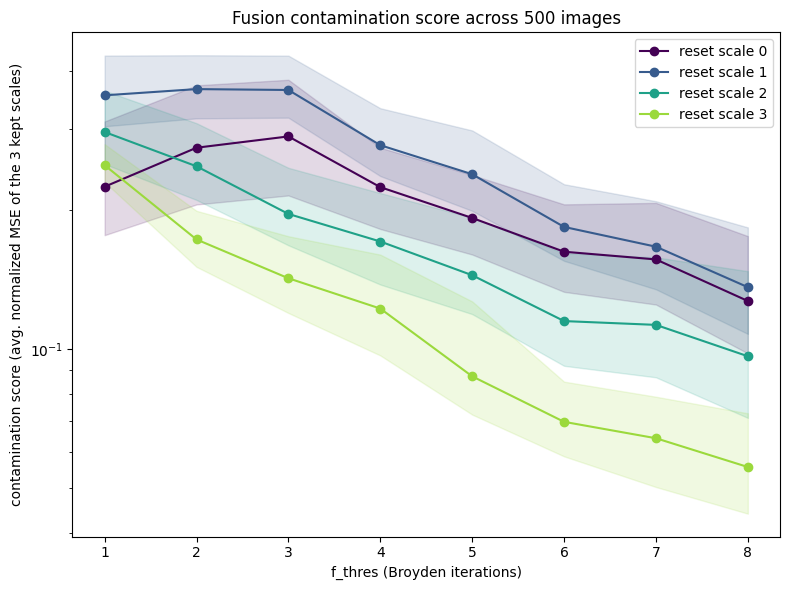
\includegraphics[width=0.8\textwidth]{informe_figuras/fig1_contaminacion_idealizado_500.png}
  \caption{Score de contaminación a través de \code{f\_thres}, experimento idealizado, 500
    imágenes. La línea es la mediana entre imágenes; la banda sombreada es el rango
    percentil 10--90.}
  \label{fig:contaminacion-idealizado}
\end{figure}

\begin{figure}[H]
  \centering
  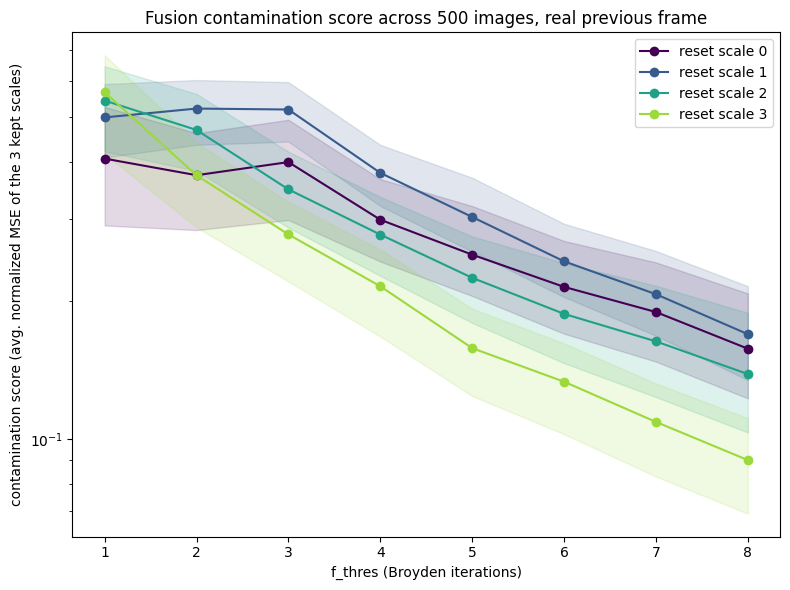
\includegraphics[width=0.8\textwidth]{informe_figuras/fig2_contaminacion_real_500.png}
  \caption{Score de contaminación a través de \code{f\_thres}, usando el cuadro real anterior de
    cada secuencia, 500 imágenes.}
  \label{fig:contaminacion-real}
\end{figure}

\subsection{Recuperación de la escala reiniciada tras una sola iteración}

Antes de la primera iteración medida (\code{f\_thres}~=~0), las 3 escalas mantenidas están, por
construcción, exactamente en $z^*$ (error cero), mientras que la escala reiniciada empieza en cero,
a una distancia de $z^*$ igual a $\overline{(z^*)^2}$ de esa escala. La Tabla~\ref{tab:recuperacion}
muestra cuánto de esa distancia inicial se recupera en una sola iteración (experimento idealizado,
500 imágenes).

\begin{table}[H]
  \centering
  \caption{Distancia de la escala reiniciada a $z^*$ en \code{f\_thres}~=~0 frente a
    \code{f\_thres}~=~1, y porcentaje recuperado en una sola iteración.}
  \label{tab:recuperacion}
  \begin{tabular}{@{}ccccc@{}}
    \toprule
    Escala & \code{f\_thres}=0 & \code{f\_thres}=1 & \% recuperado \\
    \midrule
    0 & $4.66\times10^{-3}$ & $1.60\times10^{-3}$ & 65.6\% \\
    1 & $2.63\times10^{-3}$ & $9.66\times10^{-4}$ & 63.2\% \\
    2 & $1.86\times10^{-3}$ & $7.43\times10^{-4}$ & 60.2\% \\
    3 & $1.24\times10^{-3}$ & $7.70\times10^{-4}$ & 38.1\% \\
    \bottomrule
  \end{tabular}
\end{table}

La escala~0 es la que más rápido recupera su propio error (65.6\% en una iteración), y la escala~3
la que menos (38.1\%) --- coherente con todos los demás resultados de convergencia de este proyecto.
Este dato, junto con la Tabla~\ref{tab:resultado-central}, confirma que la escala~1 no destaca por
su propia velocidad de recuperación (queda en un punto intermedio, 63.2\%): lo que la distingue es
específicamente cuánto perturba a las otras escalas al fusionarse con ellas, no qué tan rápido se
repara a sí misma.

\subsection{¿La contaminación desaparece con más iteraciones?}

La Tabla~\ref{tab:extension-27} y la Figura~\ref{fig:extension-27} muestran el score de
contaminación extendido hasta \code{f\_thres}~=~27 (una sola imagen, cuadro real anterior).

\begin{table}[H]
  \centering
  \caption{Score de contaminación extendido hasta \code{f\_thres}~=~27 (1 imagen, cuadro real
    anterior).}
  \label{tab:extension-27}
  \begin{tabular}{@{}lcccc@{}}
    \toprule
    \code{f\_thres} & Escala 0 & Escala 1 & Escala 2 & Escala 3 \\
    \midrule
    4  & 0.298 & \textbf{0.402} & 0.277 & 0.224 \\
    8  & 0.138 & \textbf{0.174} & 0.125 & 0.096 \\
    16 & 0.047 & \textbf{0.060} & 0.043 & 0.030 \\
    27 & \textbf{0.034} & 0.024 & 0.021 & 0.014 \\
    \bottomrule
  \end{tabular}
\end{table}

\begin{figure}[H]
  \centering
  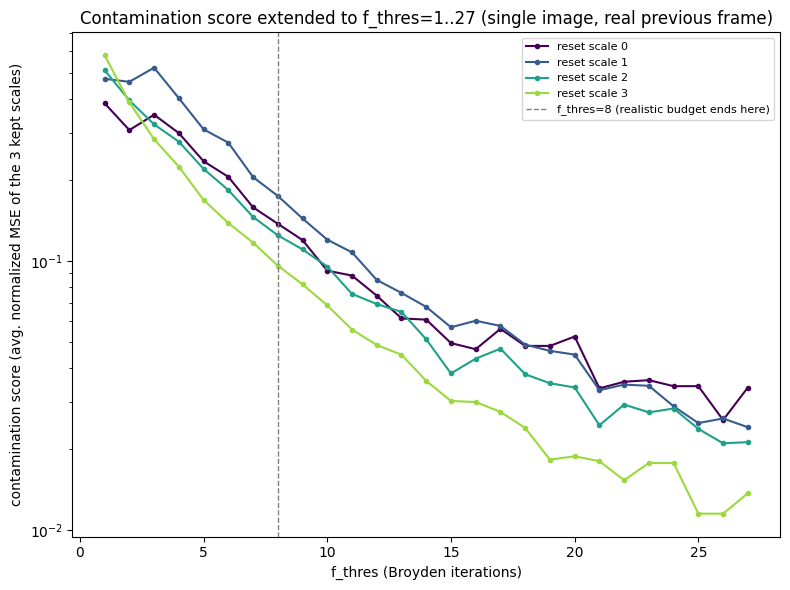
\includegraphics[width=0.75\textwidth]{informe_figuras/fig3_extendido_27_iteraciones.png}
  \caption{Score de contaminación extendido hasta \code{f\_thres}~=~27. La línea vertical punteada
    marca el límite de los presupuestos realmente usados en el sweep de streaming
    (\code{f\_thres}~$\leq$~8).}
  \label{fig:extension-27}
\end{figure}

Dos observaciones importantes. Primero, el score de todas las configuraciones cae entre 10 y 15
veces desde \code{f\_thres}~=~4 hasta 27, confirmando que la contaminación es un efecto de
presupuesto corto, no una divergencia permanente: dado suficiente tiempo, el solver sí recupera el
equilibrio verdadero sin importar qué escala se haya reiniciado. Segundo, dentro del rango realista
(\code{f\_thres}~$\leq$~8) el orden se mantiene exactamente igual que en el resto del informe
(escala~1 la peor), pero hacia \code{f\_thres}~=~27 el orden \textbf{cambia}: la escala~0 pasa a ser
la configuración con mayor contaminación, mientras que la de la escala~1 cae más rápido en el tramo
final. Esto no cambia ninguna conclusión práctica (ningún presupuesto real de streaming supera
\code{f\_thres}~=~8), pero se reporta como un hallazgo honesto y abierto, no resuelto en este
informe.

\subsection{Velocidad de convergencia por canal en el control \code{no\_reset}}

Por último, se replicó el análisis de velocidad de convergencia por canal (tasa de decaimiento,
Ecuación~\eqref{eq:tasa-decaimiento}) para la configuración de control \code{no\_reset}
(warm-start real completo, sin reiniciar nada), a nivel de las 500 imágenes. La
Tabla~\ref{tab:tasas-decaimiento} compara estos resultados contra la tasa de decaimiento
correspondiente para un arranque en frío, ya reportada en \code{convergence\_population\_analysis.ipynb}.

\begin{table}[H]
  \centering
  \caption{Tasa mediana de decaimiento por canal (unidades de $\log_{10}$ del error por
    iteración), arranque en frío frente a warm-start real, 500 imágenes.}
  \label{tab:tasas-decaimiento}
  \begin{tabular}{@{}lcccc@{}}
    \toprule
    & Escala 0 & Escala 1 & Escala 2 & Escala 3 \\
    \midrule
    Arranque en frío (cold start)   & \textbf{0.118} & 0.114 & 0.107 & 0.075 \\
    Warm-start real (\code{no\_reset}) & \textbf{0.117} & 0.099 & 0.066 & 0.030 \\
    \bottomrule
  \end{tabular}
\end{table}

El orden --- escala~0 la más rápida, escala~3 la más lenta --- se mantiene sin excepción en ambos
casos. La tasa de la escala~0 prácticamente no cambia entre arranque en frío y warm-start real
(0.118 frente a 0.117): para la escala más rápida, el tipo de arranque casi no importa. Las escalas
2 y 3, en cambio, muestran una tasa relativa menor bajo warm-start; una parte de esa diferencia es
un efecto real de arrancar ya cerca de la respuesta correcta, y otra parte es simplemente que el
ajuste aquí se hizo sobre una ventana más corta (\code{f\_thres}~=~1 a 8, en vez de 1 a 10), al ser
todo el rango disponible en esta extracción. En cualquier caso, el orden entre escalas --- que es lo
que realmente sostiene las conclusiones de este informe --- no se ve afectado.

La Figura~\ref{fig:convergencia-canal} muestra, a modo de ejemplo, la trayectoria normalizada de
cada uno de los 88 canales de la escala~0, coloreada por su propia tasa de convergencia.

\begin{figure}[H]
  \centering
  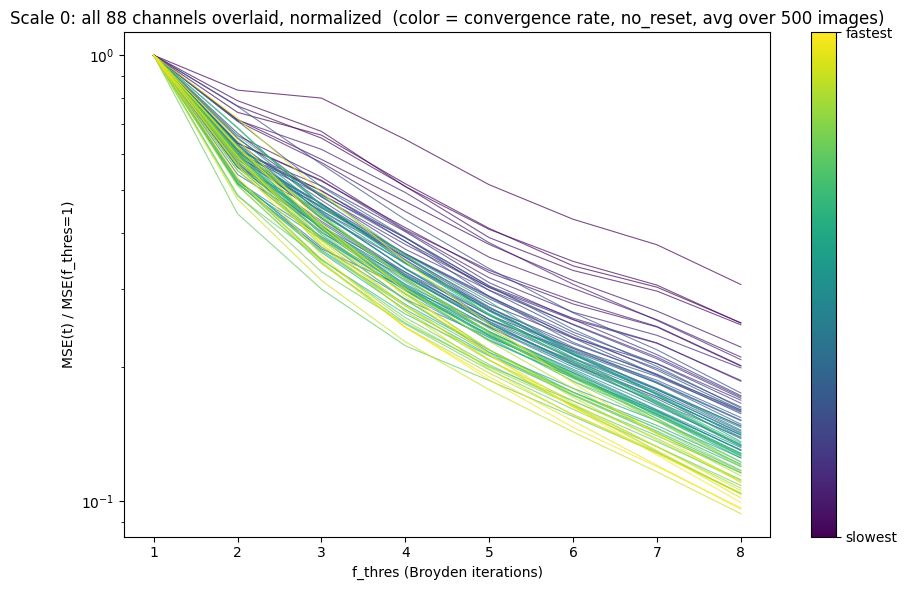
\includegraphics[width=0.75\textwidth]{informe_figuras/fig4_convergencia_canal_escala0.png}
  \caption{Escala 0: las 88 trayectorias de canal superpuestas, normalizadas por su propio valor en
    \code{f\_thres}~=~1, coloreadas por tasa de convergencia (warm-start real, 500 imágenes).}
  \label{fig:convergencia-canal}
\end{figure}

\begin{figure}[H]
  \centering
  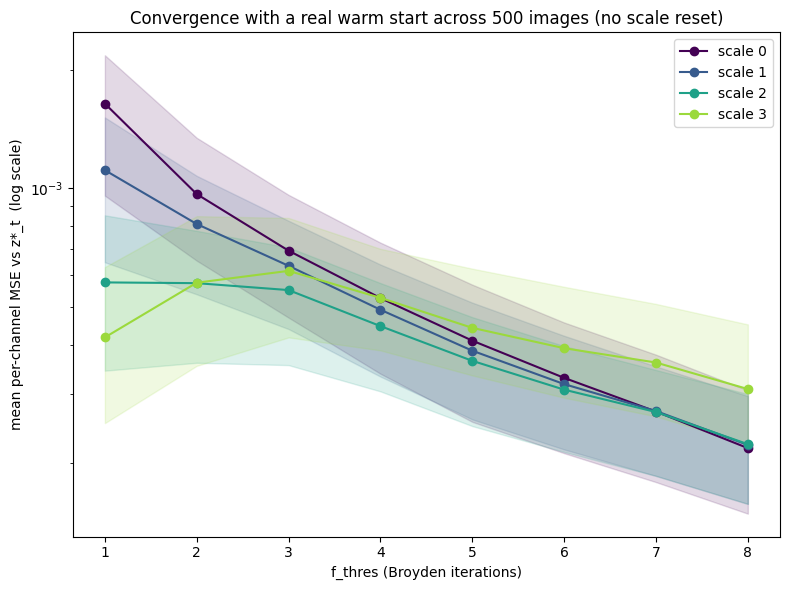
\includegraphics[width=0.75\textwidth]{informe_figuras/fig5_convergencia_no_reset_500.png}
  \caption{Convergencia con warm-start real, sin reiniciar ninguna escala, promediada sobre las 500
    imágenes (mediana y banda percentil 10--90 por escala).}
  \label{fig:convergencia-no-reset}
\end{figure}


% ============================================================
\section{Discusión}
% ============================================================

Los resultados presentados en este informe resuelven, de forma consistente en cuatro
configuraciones experimentales distintas, la contradicción planteada en la introducción. La
importancia desproporcionada de la escala~1 para el warm-start de StreamDEQ no se explica por ser
la escala más lenta en converger a su propio equilibrio --- de hecho, nunca lo es, ni en arranque en
frío ni en warm-start real, ni en una imagen ni a nivel poblacional---. En cambio, se explica por
\textbf{cuánto perturba a las otras 3 escalas} al fusionarse con ellas en cada iteración del
solver: reiniciar la escala~1 deja a las escalas 0, 2 y 3 sistemáticamente más lejos de su propio
equilibrio que si se hubiera reiniciado cualquier otra escala.

Este resultado se sostiene tanto en el entorno idealizado (que aísla la fusión de cualquier
variación de contenido entre cuadros) como con cuadros de video genuinamente distintos, y tanto en
una imagen aislada como en las 500 imágenes de validación de Cityscapes --- descartando que se trate
de una coincidencia de una sola imagen o de un artefacto de la simplificación idealizada.

El hallazgo del cambio de orden en \code{f\_thres}~=~27 (Sección~\ref{sec:resultados}) es un
recordatorio importante: la afirmación ``reiniciar la escala~1 es lo peor'' es válida
específicamente \textbf{dentro del rango de presupuestos que StreamDEQ usa en la práctica}
(\code{f\_thres}~$\leq$~8), no como una propiedad universal del modelo en cualquier régimen de
iteraciones. Fuera de ese rango, la dinámica de recuperación es distinta y no se explora más a
fondo en este informe.


% ============================================================
\section{Conclusiones}
% ============================================================

\begin{enumerate}[leftmargin=*]
  \item La importancia de la escala~1 para el warm-start de StreamDEQ, encontrada en el sweep
    original de mIoU, tiene una explicación mecanicista concreta: la contaminación que produce por
    fusión sobre las otras 3 escalas, no su propia velocidad de convergencia.
  \item Este resultado se verificó en 4 configuraciones experimentales independientes (idealizado
    o con cuadro real, una imagen o 500 imágenes), obteniendo siempre el mismo orden entre escalas:
    reiniciar la escala~1 es lo más perjudicial, seguida de la escala~0, luego la escala~2, y por
    último la escala~3.
  \item El uso de cuadros de video reales (en vez de la simplificación idealizada) confirma que el
    efecto no depende de esa idealización, aunque sí añade una pequeña cantidad de error de base
    proveniente de la deriva natural de contenido entre cuadros consecutivos.
  \item La contaminación es un efecto transitorio: dado un presupuesto de iteraciones lo bastante
    grande (\code{f\_thres}~=~27), el score de contaminación de las 4 configuraciones cae entre 10 y
    15 veces respecto a \code{f\_thres}~=~4, aunque el orden entre configuraciones deja de ser
    estable fuera del rango de presupuestos realmente usado en producción.
  \item El orden de velocidad de convergencia entre escalas (0 la más rápida, 3 la más lenta) es una
    propiedad estructural de la arquitectura --- se mantiene igual sin importar si el arranque es en
    frío o en warm-start real, y si se mide en una sola imagen o promediado sobre 500.
\end{enumerate}


% ============================================================
\section{Trabajo futuro}
% ============================================================

Quedan dos extensiones naturales, no abordadas en este informe:

\begin{itemize}
  \item \textbf{Cadena recursiva fiel al artículo original.} Todos los experimentos con cuadro real
    anterior de este informe usan un $z^*_{t-1}$ calculado con 27 iteraciones limpias, un punto de
    partida mejor de lo que StreamDEQ real jamás tiene disponible: en producción, el estado que se
    pasa de un cuadro a otro proviene siempre de una cadena recursiva de soluciones parciales, cada
    una resuelta con el mismo presupuesto pequeño de iteraciones (\code{f\_thres} = 1, 2, 4 u 8),
    empezando desde cero en el primer cuadro de cada secuencia. Replicar esa cadena recursiva
    exacta --- reutilizando el mecanismo real de \code{self.prev\_outs} del modelo en vez de un
    $z^*_{t-1}$ idealizado --- permitiría comparar directamente estos resultados contra el
    comportamiento genuino de StreamDEQ en producción.
  \item \textbf{De diagnóstico a método.} Este informe explica \emph{por qué} ocurre el problema,
    pero no propone todavía una corrección. Un paso natural sería diseñar un esquema de
    inicialización que trate a la escala~1 con más cuidado que las demás (por ejemplo, sin
    ponerla nunca en cero por completo, o dándole iteraciones adicionales cuando su estado se
    considere obsoleto) y medir si eso mejora el mIoU o la velocidad del streaming real frente al
    StreamDEQ original --- convirtiendo así el diagnóstico en una contribución con una mejora
    cuantificable, no solo una explicación.
\end{itemize}


% ============================================================
\section*{Reproducibilidad}
% ============================================================

Todos los experimentos descritos en este informe están implementados en
\code{results/ml\_project/fusion\_contamination.ipynb}, dentro del repositorio del proyecto. Los
scripts de extracción poblacional usados son:
\begin{itemize}
  \item \code{scripts/ml\_project/extract\_fusion\_contamination.py} --- experimento idealizado,
    500 imágenes.
  \item \code{scripts/ml\_project/extract\_zstar\_prev\_frame.py} --- equilibrio del cuadro real
    anterior, 500 secuencias.
  \item \code{scripts/ml\_project/extract\_fusion\_contamination\_realprev.py} --- experimento con
    cuadro real anterior, 500 imágenes.
\end{itemize}
Todos los scripts son reanudables (omiten imágenes ya procesadas) y están documentados con más
detalle en \code{README\_ML\_PROJECT.md}.

\end{document}
